\chapter{}
\label{lecture3}
\section[Функционалы, зависящие от старших производных (продолжение).]{Вариационные задачи для функционалов, зависящих от старших производных (продолжение).}
\label{lecture3section1}
\markboth{Лекция~\thechapter.}{\thesection\quad Функционалы, зависящие от старших производных.}
Итак, мы рассматриваем функционал 
\begin{equation}
	\label{l3:eq:1}
	\J[y]=\int\limits_a^b F(x,y,y',y'')\,dx.
\end{equation}
Считаем, что $F\in\Cfn{3}$, $x\in[a,b]$, $|y|<M,\ \forall y',\ y''$. 
Будем искать минимум функционала \eqref{l3:eq:1} в классе функций
\begin{multline*}
	\K=\Big\{y(x)\Big|\,y\in\Cfn[{[a,b]}]{2},\ y(a)=y_0,\,y'(a)=y'_0,\\ y(b)=y_1,\,y'(b)=y'_1,\ |y|<M\Big\}.
\end{multline*}
Как обычно предполагаем, что минимайзер существует. Обозначим его через $y$ и введём понятие допустимого изменения $\eta(x)$ по аналогии с предыдущими случаями.
\begin{Def}
	$\eta(x)$ --- \textbf{допустимое изменение}, если 
	\begin{equation*}
		\tilde{y}\eqdef y+t\cdot\eta\in\K,\quad\text{при }|t|\ll1.
	\end{equation*}
\end{Def}
\noindent Отсюда 
\begin{gather*}
	\eta=\dfrac{\tilde{y}-y}t
	\intertext{и поэтому}
	\eta\in\Cfn[{[a,b]}]{2},\quad \eta(a)=\eta'(a)=\eta(b)=\eta'(b)=0.
\end{gather*}
Далее 
\begin{equation}
	\label{l3:eq:2}
	\J[y+t\cdot\eta]\geqslant\J[y],\quad|t|\ll1,
\end{equation}
и, полагая $\phi(t)=\J[y+t\cdot\eta]$, видим, что 
\begin{equation}
	\label{l3:eq:3}
	\phi(t)\geqslant\phi(0).
\end{equation}
Так как $t=0$ --- точка минимума для функции $\phi(t)$, то должно выполняться необходимое условие минимума.
\begin{equation}\label{l3:eq:4}
	\phi'(0)=0,
\end{equation}
то есть
\begin{equation}\label{l3:eq:5}
	\left.\der{}{t}\J[y+t\cdot\eta]\right|_{t=0}=0.
\end{equation}
Дадим истолкование левым частям \eqref{l3:eq:4}, \eqref{l3:eq:5}, не предполагая, что $\eta$~--- допустимое изменение, а считая только $\eta\in\Cfn[{[a,b]}]{2}$. Тогда по формуле Тейлора
\begin{equation*}
	\phi(t)=\phi(0)+t\cdot\phi'(0)+o(t)
\end{equation*}
и
\begin{equation*}
	\phi(t)-\phi(0)=t\cdot\phi'(0)+o(t).
\end{equation*}
Соответственно
\begin{equation*}
	\J[y+t\cdot\eta]=\J[y]+t\cdot\left.\der{}{t}\J[y+t\cdot\eta]\right|_{t=0}+o(t)
\end{equation*}
и
\begin{equation*}
	\J[y+t\cdot\eta]-\J[y]=t\cdot\left.\der{}{t}\J[y+t\cdot\eta]\right|_{t=0}+o(t).
\end{equation*}
Назовём величину $t\cdot\left.\displaystyle\der{}{t}\J[y+t\cdot\eta]\right|_{t=0}$ \emph{первой вариацией} и обозначим через $\delta\J$. Таким образом первая вариация --- это главная часть приращения функционала $\J[y]$ при замене $y$ на $y+t\cdot\eta$. Из~\eqref{l3:eq:5} следует, что если $y$ --- минимайзер (или максимайзер --- рассуждения не меняются), то 
\begin{equation}
	\label{l3:eq:6}
	\delta\J=0.
\end{equation}

Найдём выражение для первой вариации. Имеем
\begin{multline*}
	\delta\J=t\cdot\left.\der{}{t}\J[y+t\cdot\eta]\right|_{t=0}=\\=t\cdot\left.\der{}{t}\int\limits_a^b F(x,y+t\cdot\eta,y'+t\cdot\eta',y''+t\cdot\eta'')\,dx\right|_{t=0}.
\end{multline*}
Вводим обычные обозначения $\tilde{y}\eqdef y+t\cdot\eta$, $\widetilde{F}\eqdef F(x,\tilde{y},\tilde{y}',\tilde{y}'')$. Тогда 
\begin{multline*}
	\delta\J=t\cdot\left.\int\limits_a^b\left( \widetilde{F}_{\tilde{y}}\cdot\eta+\widetilde{F}_{\tilde{y}'}\cdot\eta'+\widetilde{F}_{\tilde{y}''}\cdot\eta''\right)\,dx\right|_{t=0}=\\=t\cdot\int\limits_a^b \left(F_{y}\cdot\eta+F_{y'}\cdot\eta'+F_{y''}\cdot\eta''\right)\,dx.
\end{multline*}
Как уже говорилось раньше, надо избавиться от $\eta'$, $\eta''$ под знаком интеграла. Сделаем это, проведя интегрирование по частям. При этом мы будем использовать повышенную гладкость минимайзера. Имеем
\begin{equation*}
	\int\limits_a^b \underbrace{F_{y'}}_{u}\cdot\underbrace{\eta'\,dx}_{dv}=F_{y'}\cdot\eta\mathop{\Big|}\limits_a^b-\int\limits_a^b\der{}{x}F_{y'}\cdot\eta\,dx,
\end{equation*}
\begin{multline*}
	\int\limits_a^b \underbrace{F_{y''}}_{u}\cdot\underbrace{\eta''\,dx}_{dv}=F_{y''}\cdot\eta'\mathop{\Big|}\limits_a^b-\int\limits_a^b\underbrace{\der{}{x}F_{y''}}_{u}\cdot\underbrace{\eta'\,dx}_{dv}=\\=\left(F_{y''}\cdot\eta'-\der{}{x}F_{y''}\cdot\eta\right)\mathop{\Big|}\limits_a^b+\int\limits_a^b\dder{}{x}F_{y''}\cdot\eta\,dx.
\end{multline*}
Подставляя эти результаты в выражение для $\delta\J$, получим 
\begin{multline}
	\label{l3:eq:B}
	\delta\J=t\cdot\left[\vphantom{\int\limits_a^b}\left(F_{y'}\cdot\eta+F_{y''}\cdot\eta'-\der{}{x}F_{y''}\cdot\eta\right)\mathop{\Big|}\limits_a^b+\right.\\\left.+\int\limits_a^b\left(F_{y}-\der{}{x}F_{y'}+\dder{}{x}F_{y''}\right)\cdot\eta\,dx\right].\tag{B}
\end{multline}
Это главная часть приращения функционала $\J[y]$ при замене $y$ на $y\?+t\cdot\eta$. Мы её вывели при $y\in\Cfn{4}$. Для этой формулы введено обозначение \eqref{l3:eq:B}, так как формула \eqref{l1:eq:A} была на \hyperref[lecture1]{первой лекции}, но для $F=F(x,y,y')$. 

Пусть $\eta$ --- допустимое изменение. Тогда в силу \eqref{l3:eq:6} приравнивая $\delta\J=0$, мы получаем уравнение, из которого с помощью леммы Лагранжа выведем уравнение для минимайзера. Так как $\eta$ --- допустимое изменение, то $\eta=\eta'=0$, при $x=a,b$ поэтому внеинтегральных членов в $\delta\J$ не будет и равенство $\delta\J=0$ влечёт соотношение 
\begin{equation*}
	\int\limits_a^b\left(F_{y}-\der{}{x}F_{y'}+\dder{}{x}F_{y''}\right)\cdot\eta\,dx=0,\quad\forall\eta\text{ --- допустимое.}
\end{equation*}
Откуда с помощью леммы Лагранжа получим для минимайзера \emph{уравнение Эйлера--Пуассона}:
\begin{equation}
	\label{l3:eq:7}
	 F_{y}-\der{}{x}F_{y'}+\dder{}{x}F_{y''}=0.
\end{equation}
Это обыкновенное дифференциальное уравнение четвёртого порядка и его решение $y\?=y(x,c_1,c_2,c_3,c_4)$.

Из граничных условий в общем случае константы $c_1,\ldots,c_4$ можно найти:
\begin{multline*}
	 y_0=y(a,c_1,\ldots,c_4),\ y'_0=y'(a,c_1,\ldots,c_4),\\ y_1=y(b,c_1,\ldots,c_4),\ y'_1=y'(b,c_1,\ldots,c_4).
\end{multline*}

Для простоты мы ограничились случаем, когда интегрант зависит от производных только первого и второго порядка. Но на этом же пути можно рассмотреть случай, когда интегрант зависит от производных любого порядка. Приведём без доказательства полученные результаты.
\begin{multline*}
	\J[y]=\int\limits_a^b F(x,y,y',\ldots,y^{(n)})\,dx,\\ F\in\Cfn{n+1},\ x\in[a,b],\ |y|<M,\ y',\ldots,y^{(n)}\text{ --- любые},\\
	\K=\left\{y(x)|y\in\Cfn[{[a,b]}]{n},\ y^{(j)}(a)=y_0^{(j)},\ y^{(j)}(b)=y_1^{(j)},\ j=\overline{0,n-1}\right\},
\end{multline*}
здесь $y^{(0)}(x)\equiv y(x)$, $y_0^{(j)}$ и $y_1^{(j)}$ --- произвольные фиксированные константы. Тогда минимайзер в задаче на $\min\limits_{y\in\K}\J[y]$ удовлетворяет уравнению 
\begin{equation}
	\label{l3:eq:8}
	 F_y-\der{}{x}F_{y'}+\dder{}{x}F_{y''}-\ldots+(-1)^{n}\der{^n}{x^n}F_{y^{(n)}}=0,
\end{equation} 
решение которого ищется в классе
$y\in\Cfn[{[a,b]}]{2n}$, $y^{(j)}(a)=y_0^{(j)}$,  $y^{(j)}(b)=y_1^{(j)}$, $j=\overline{0,n-1}$.

Разумеется всё, что мы говорили о решениях уравнений Эйлера--Лагранжа, мы повторяем и здесь: если экстремайзер существует, то мы его ищем, решая \eqref{l3:eq:8}. Если о его существовании ничего не известно, то решение \eqref{l3:eq:8} --- кривая, подозрительная на экстремум. Если \eqref{l3:eq:8} не имеет решений, то экстремайзера нет. Исследование знака второй вариации подсказывает, чем может являться найденная экстремаль (точнее~--- чем не может\dots)

Возвратимся к задаче о равновесии балки. Мы получили там функционал 
\begin{equation*}
	 E[y]=\int\limits_{-l}^{+l}\left(g\cdot\rho\cdot y+\frac12\cdot\mu\cdot y^{\prime\prime2}\right)\,dx,
\end{equation*}
где $g$, $\rho$, $\mu$ --- постоянные.
Уравнение Эйлера--Пуассона 
\begin{equation*}
	 g\cdot\rho+\mu\cdot y^{IV}=0,
\end{equation*}
откуда
\begin{equation*}
	 y(x)=-\frac{g\cdot\rho}{4!\cdot\mu}\cdot x^4+c_1\cdot x^3+c_2\cdot x^2+c_3\cdot x+c_4.
\end{equation*}
Используя граничные условия $y(-l)=y(+l)=y'(-l)=y'(+l)=0$ получим
\begin{equation*}
	 y=-\frac{g\cdot\rho}{24\cdot\mu}(x-l)^2\cdot(x+l)^2.
\end{equation*} 

\section[Задачи со свободными концами.]{Вариационные задачи со свободной границей для функционалов, зависящих от функций одной переменной.}
\label{lecture3section2}
До сих пор мы рассматривали вариационные задачи, в которых допустимые функции принимали заданные значения на границах отрезка. Но это вовсе не обязательно. Вернёмся к задаче о брахистохроне. Мы установили, что время скатывания материальной точки с высоты $y_0$ по кривой $y(x)$ до правой стенки 
\begin{equation*}
	 T[y]=\int\limits_a^b\frac{\sqrt{1+y^{\prime2}}}{\sqrt{2\cdot g\cdot(y_0-y)}}\,dx.
\end{equation*}
\begin{figure}[H]\centering
\tikzset{every picture/.style={line width=0.75pt}} %set default line width to 0.75pt        

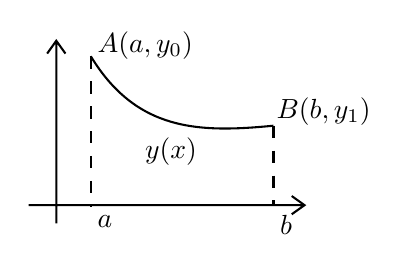
\begin{tikzpicture}[x=0.75pt,y=0.75pt,yscale=-0.88,xscale=0.88]
	%uncomment if require: \path (0,142); %set diagram left start at 0, and has height of 142
	
	%Shape: Axis 2D [id:dp5296256236644323] 
	\draw  (57,105) -- (208,105)(72.1,15) -- (72.1,115) (201,100) -- (208,105) -- (201,110) (67.1,22) -- (72.1,15) -- (77.1,22)  ;
	%Curve Lines [id:da5139961929878707] 
	\draw    (91,23.5) .. controls (116,64.5) and (150,65.5) .. (191,61.5) ;
	%Straight Lines [id:da7749819981896289] 
	\draw  [dash pattern={on 4.5pt off 4.5pt}]  (91,23.5) -- (91,105.5) ;
	%Straight Lines [id:da17627525123267485] 
	\draw  [dash pattern={on 4.5pt off 4.5pt}]  (191,61.5) -- (191,105.5) ;
	
	% Text Node
	\draw (93,108.9) node [anchor=north west][inner sep=0.75pt]    {$a$};
	% Text Node
	\draw (193,108.9) node [anchor=north west][inner sep=0.75pt]    {$b$};
	% Text Node
	\draw (93,8.4) node [anchor=north west][inner sep=0.75pt]    {$A( a,y_{0})$};
	% Text Node
	\draw (191,44.4) node [anchor=north west][inner sep=0.75pt]    {$B( b,y_{1})$};
	% Text Node
	\draw (119,66.4) node [anchor=north west][inner sep=0.75pt]    {$y( x)$};
	
	
\end{tikzpicture}
\caption{~}
\label{l3:fig:1}
\end{figure}
Мы искали минимум функционала по траекториям, для которых были заданы начальная и конечная точки. Но можно поставить задачу по-другому: не задавать конечную точку! И тогда класс $\K$ допустимых кривых будет выглядеть так:
\begin{equation*}
	\K=\left\{y(x)\middle|y\in\Cfn[{[a,b]}]{1},\ y(a)=y_0,\ |y|<M\right\}.
\end{equation*}
Найти $\displaystyle\min\limits_{y\in\K}\,T[y]$.

Переходим к общему случаю. Пусть функционал $\J[y]$ тот же, что в \hyperref[lecture1]{первой лекции}
\begin{multline*}
	\J[y]=\int\limits_a^b F(x,y,y')\,dx,\quad
	F\in\Cfn{2},\ x\in[a,b],\ |y|<M,\ \forall y';\\ \K=\left\{y(x)\middle|y\in\Cfn[{[a,b]}]{1},\ |y|<M\right\}.
\end{multline*}
Допустимы любые кривые класса $\Cfn[{[a,b]}]{1}$, $|y|<M$.
\begin{figure}[H]\centering
\tikzset{every picture/.style={line width=0.75pt}} %set default line width to 0.75pt        

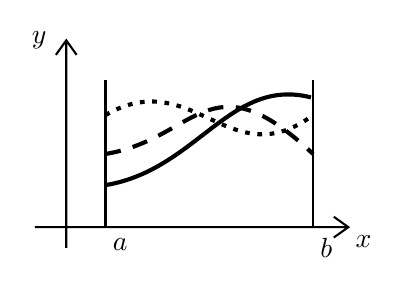
\begin{tikzpicture}[x=0.75pt,y=0.75pt,yscale=-1,xscale=1]
	%uncomment if require: \path (0,142); %set diagram left start at 0, and has height of 142
	
	%Shape: Axis 2D [id:dp686169032500981] 
	\draw  (57,105) -- (208,105)(72.1,15) -- (72.1,115) (201,100) -- (208,105) -- (201,110) (67.1,22) -- (72.1,15) -- (77.1,22)  ;
	%Curve Lines [id:da9286352692192188] 
	\draw [line width=1.5]  [dash pattern={on 1.69pt off 2.76pt}]  (91,51) .. controls (133,26.5) and (151,81) .. (191,51) ;
	%Straight Lines [id:da14648037004429826] 
	\draw    (91,34) -- (91,105.5) ;
	%Straight Lines [id:da6289208427845525] 
	\draw    (191,34) -- (191,105.5) ;
	%Curve Lines [id:da63694563394428] 
	\draw [line width=1.5]  [dash pattern={on 5.63pt off 4.5pt}]  (91,69.75) .. controls (135,62.5) and (141,22.5) .. (191,69.75) ;
	%Curve Lines [id:da6807862818346342] 
	\draw [line width=1.5]    (91,84.75) .. controls (135,77.5) and (151,32.5) .. (190,42.5) ;
	
	% Text Node
	\draw (93,108.9) node [anchor=north west][inner sep=0.75pt]    {$a$};
	% Text Node
	\draw (193,108.9) node [anchor=north west][inner sep=0.75pt]    {$b$};
	% Text Node
	\draw (210,107.4) node [anchor=north west][inner sep=0.75pt]    {$x$};
	% Text Node
	\draw (54,9.4) node [anchor=north west][inner sep=0.75pt]    {$y$};
	
	
\end{tikzpicture}
\caption{~}
\label{l3:fig:2}
\end{figure}
Пусть $y$ --- минимайзер в задаче на $\min\limits_{y\in\K}\,\J[y]$. Функция $\eta$ --- допустимое изменение, если
\begin{equation*}
	\tilde{y}\eqdef y+t\cdot\eta\in\K,\quad |t|\ll1.
\end{equation*}
Отсюда следует, что единственное ограничение на $\eta$ --- требование гладкости: $\eta(x)\in\Cfn[{[a,b]}]{1}$. Рассуждая стандартным образом, мы получим, что необходимое условие экстремума --- это обращение в ноль первой вариации. Выражение для первой вариации даётся равенством \eqref{l1:eq:A} \hyperref[lecture1]{первой лекции}. Перепишем его 
\begin{equation}
	\label{l3:eq:9}
	 \delta\J=t\left\{\int\limits_a^b\left(F_y-\der{}{x}F_{y'}\right)\cdot\eta\,dx+F_{y'}\cdot\eta\mathop{\Big|}\limits_a^b\right\}.
\end{equation}
Так как $y$ --- экстремайзер, то $\delta\J=0$, при $\forall\eta$ --- допустимом. Возьмём $\eta(a)=\eta(b)=0$. Тогда из равенства $\delta\J=0$ получим 
\begin{equation*}
	\int\limits_a^b\left(F_y-\der{}{x}F_{y'}\right)\cdot\eta\,dx=0,\quad \forall\eta\in\Cfn[{[a,b]}]{1},\ \eta(a)=\eta(b)=0.
\end{equation*}
Отсюда в силу леммы Лагранжа получаем уравнение Эйлера
\begin{equation}
	\label{l3:eq:10}
	 F_{y}-\der{}{x}F_{y'}=0.
\end{equation}
Уравнение \eqref{l3:eq:10} не зависит от выбора $\eta$ ($\eta$  туда не входит). Поэтому в силу \eqref{l3:eq:9} для любых $\eta$
\begin{equation*}
	\delta\J=t\cdot F_{y'}\cdot\eta\mathop{\Big|}\limits_a^b=0.
\end{equation*}
Взяв сначала $\eta(b)=1$, $\eta(a)=0$ получим $F_{y'}\big|_{x=b}=0$; при $\eta(b)=0$, $\eta(a)=1$ получим $F_{y'}\big|_{x=a}=0$. Таким образом несмотря на отсутствие граничных условий в классе допустимых функций \K, экстремайзер должен удовлетворять так называемым \emph{естественным граничным условиям} (ЕГУ)
\begin{equation}
	\label{l3:eq:11}
	 F_{y'}(a,y(a),y'(a))=0;\ F_{y'}(b,y(b),y'(b))=0.
\end{equation}  
Разумеется, если на каком-то конце отрезка граничные условия заданы, то на этом конце ЕГУ отсутствует.

Рассмотрим важный частный случай
\begin{equation*}
	F=\frac{A(x,y)}{\sqrt{1+y^{\prime 2}}},\quad A(x,y)>0.
\end{equation*}
В этом случае на свободном конце ЕГУ
\begin{equation*}
	-\frac12\cdot\frac{A(x,y)\cdot2\cdot y'}{(1+y^{\prime2})^{3/2}}=0\quad\Rightarrow\quad y'=0.
\end{equation*} 
То есть траектория ортогональна к границе.

Варианты с неполным заданием граничных условий могут быть и в случае функционалов, зависящих от старших производных. Рассмотрим
\begin{equation*}
	\J[y]=\int\limits_a^b F(x,y,y',y'')\,dx.
\end{equation*}
Мы решали задачу на 
\begin{gather*}
\min\limits_{y\in\K}\,\J[y],\intertext{где}\K=\left\{y(x)\middle|y\in\Cfn[{[a,b]}]{2},\ y(a),\,y'(a),\,y(b),\,y'(b)\text{ --- заданы}\right\}.
\end{gather*}

Давайте рассмотрим теперь класс допустимых функций 
\begin{equation*}
	\K=\left\{y(x)\middle|y\in\Cfn[{[a,b]}]{2},\ y(a)=y_0,\,y'(b)=y_1^{(1)},\ |y|<M\right\}.
\end{equation*}
Таким образом в отличие от рассмотренного ранее случая свободны $y'(a)$ и $y(b)$. Пусть $\eta(x)\in\Cfn[{[a,b]}]{2}$. Мы находим главную часть приращения 
\begin{equation*}
	\J[y+t\cdot\eta]-\J[y]=\delta\J+o(t),
\end{equation*}
где $\delta\J$ даётся равенством \eqref{l3:eq:B} \hyperref[lecture3]{текущей лекции} (на стр.~\pageref{l3:eq:B}). 

Функция $\eta(x)$ --- допустимое изменение для задачи $\min\limits_{y\in\K}\,\J[y]$, если
\begin{equation*}
	\tilde{y}\eqdef y+t\cdot\eta\in\K,\quad t\ll1.
\end{equation*}
Так как
\begin{gather*}
	\eta=\dfrac{\tilde{y}-y}{t},
	\intertext{то}
	\eta(a)=0,\ \eta'(b)=0.
\end{gather*}
Значения $\eta'(a)$ и $\eta(b)$ --- свободны. Разумеется, $\eta\in\Cfn[{[a,b]}]{2}$. Условие экстремума: $\delta\J=0$ при допустимых $\eta$. Так как не запрещено взять $\eta(a)=\eta'(a)=\eta(b)=\eta'(b)=0$, то как и раньше в силу \eqref{l3:eq:B}\footnote{\begin{multline*}
		\delta\J=t\cdot\left[\vphantom{\int\limits_a^b}\left(F_{y'}\cdot\eta+F_{y''}\cdot\eta'-\der{}{x}F_{y''}\cdot\eta\right)\mathop{\Big|}\limits_a^b+\right.\\\left.\int\limits_a^b\left(F_{y}-\der{}{x}F_{y'}+\dder{}{x}F_{y''}\right)\cdot\eta\,dx\right].\tag{B}
\end{multline*}} получим для минимайзера $y(x)$ уравнение
\begin{equation*}
	 F_y-\der{}{x}F_{y'}+\dder{}{x}F_{y''}=0.
\end{equation*}
Поэтому в формуле первой вариации в случае минимайзера останутся только внеинтегральные члены, которые должны равняться нулю. Имеем
\begin{equation}
	\label{l3:eq:12}
	\left(F_{y'}-\der{}{x}F_{y''}\right)\cdot\eta\mathop{\Big|}\limits_a^b+F_{y''}\cdot\eta'\mathop{\Big|}\limits_a^b=0.
\end{equation}
Так как $\eta(a)=0$ и $\eta'(b)=0$, то из \eqref{l3:eq:12} получим
\begin{equation}
	\label{l3:eq:13}
	\left(F_{y'}-\der{}{x}F_{y''}\right)\Big|_{x=b}\cdot\eta(b)-F_{y''}\Big|_{x=a}\cdot\eta'(a)=0.
\end{equation}
Отсюда полагая сначала $\eta'(a)=0$, $\eta(b)=1$ имеем
\begin{equation}
	\label{l3:eq:14}
	\left(F_{y'}-\der{}{x}F_{y''}\right)\Big|_{x=b}=0,
\end{equation}
a потом при $\eta'(a)=1$, $\eta(b)=0$ получим 
\begin{equation}
	\label{l3:eq:15}
	 F_{y''}\Big|_{x=a}=0.
\end{equation}
\eqref{l3:eq:14} и \eqref{l3:eq:15} --- это ЕГУ в данном случае.

Прежде чем переходить к другому типу задач, вернёмся к стандартной задаче со свободной границей, но вместо функционала
\begin{equation*}
	\J[y]=\int\limits_a^b F(x,y,y')\,dx
\end{equation*}
рассмотрим функционал
\begin{equation}
	\label{l3:eq:16}
	\widehat{\J}[y]=\int\limits_a^b F(x,y,y')\,dx+d_1\cdot y^2(a)+d_2\cdot y^2(b),
\end{equation}
где $d_1\geqslant0$, $d_2\geqslant0$ --- фиксированные константы. Раньше мы не могли рассматривать подобные функционалы, поскольку $y(a)$ и $y(b)$ были заданы и добавка $d_1\cdot y^2(a)+d_2\cdot y^2(b)$ являлась бы фиксированным числом, не зависящим от $y(x)$. Но теперь у нас $y(a)$ и $y(b)$ не заданы и значение $\widehat{\J}[y]$ зависит от них. Пусть
\begin{equation*}
	\K=\left\{y(x)\middle|y\in\Cfn[{[a,b]}]{1},\ |y|<M\right\},\ \eta\in\Cfn[{[a,b]}]{1}.
\end{equation*}
Тогда как и раньше $\tilde{y}=y+t\cdot\eta\in\K$, при $y\in\K,\ t\ll1$. Если $y$ --- минимайзер, то 
\begin{equation*}
	\left.\der{}{t}\widehat{\J}[y+t\cdot\eta]\right|_{t=0}=0,
\end{equation*}
то есть в силу \eqref{l3:eq:9}
\begin{equation}
	\label{l3:eq:17}
	\int\limits_a^b\left(F_y-\der{}{x}F_{y'}\right)\cdot\eta\,dx+F_{y'}\cdot\eta\mathop{\Big|}\limits_a^b+2\cdot d_1\cdot y(a)\cdot\eta(a)+2\cdot d_2\cdot y(b)\cdot\eta(b)=0.
\end{equation}
Отсюда при $\eta(a)=\eta(b)=0$ получаем как и раньше уравнение Эйлера
\begin{equation*}
	 F_y-\der{}{y}F_{y'}=0.
\end{equation*}
и поэтому \eqref{l3:eq:17} запишется в виде 
\begin{equation}
	\label{l3:eq:18}
	\left(F_{y'}+2\cdot d_2\cdot y\right)\cdot\eta\Big|_{x=b}+\left(-F_{y'}+2\cdot d_1\cdot y\right)\cdot\eta\Big|_{x=a}=0.
\end{equation}
Из~\eqref{l3:eq:18} сначала при $\eta(a)=1$, $\eta(b)=0$, а потом при $\eta(a)=0$, $\eta(b)=1$ получим ЕГУ для данного случая
\begin{equation}
	\label{l3:eq:19}
	 F_{y'}(b,y(b),y'(b))=-2\cdot y(b)\cdot d_2,\ F_{y'}(a,y(a),y'(a))=2\cdot y(a)\cdot d_1.
\end{equation}
Пример, когда возникают функционалы вида \eqref{l3:eq:16}, будет приведён позже.

\section{Задачи с <<подвижными концами>>.}
\label{lecture3section3}
В рассмотренных нами случаях появления естественных граничных условий интервал, на котором были заданы допустимые функции, это $[a,b]$. Однако есть целый ряд задач, в которых интервал не задан, ибо он может быть разным для разных допустимых функций. Такая ситуация возникает, когда концы кривых, отвечающих допустимым функциям $y(x)$, лежат на некоторых заданных фиксированных кривых. Рассмотрим пример. 

Пусть в плоской среде со скоростью распространения света $v(x,y)$ заданы две кривые $y_1=f_1(x)$, $y_2=f_2(x)$.
\begin{figure}[H]\centering
\tikzset{every picture/.style={line width=0.75pt}} %set default line width to 0.75pt        

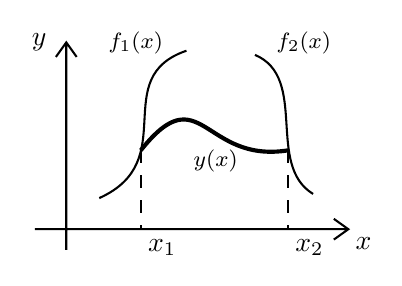
\begin{tikzpicture}[x=0.75pt,y=0.75pt,yscale=-1,xscale=1]
	%uncomment if require: \path (0,142); %set diagram left start at 0, and has height of 142
	
	%Shape: Axis 2D [id:dp6276133102920212] 
	\draw  (57,105) -- (208,105)(72.1,15) -- (72.1,115) (201,100) -- (208,105) -- (201,110) (67.1,22) -- (72.1,15) -- (77.1,22)  ;
	%Curve Lines [id:da72925318150536] 
	\draw [line width=0.75]    (88,90) .. controls (128,72) and (92,32) .. (130,19) ;
	%Straight Lines [id:da5118863835432821] 
	\draw  [dash pattern={on 4.5pt off 4.5pt}]  (108,67) -- (108,105) ;
	%Curve Lines [id:da7558847164287084] 
	\draw [line width=0.75]    (191,88) .. controls (168,74) and (189,32) .. (163,21) ;
	%Straight Lines [id:da6236180023236073] 
	\draw  [dash pattern={on 4.5pt off 4.5pt}]  (179,67) -- (179,105) ;
	%Curve Lines [id:da2748569708703843] 
	\draw [line width=1.5]    (108,67) .. controls (137,30.5) and (138,73.5) .. (179,67) ;
	
	% Text Node
	\draw (110,108.4) node [anchor=north west][inner sep=0.75pt]    {$x_{1}$};
	% Text Node
	\draw (210,107.4) node [anchor=north west][inner sep=0.75pt]    {$x$};
	% Text Node
	\draw (54,9.4) node [anchor=north west][inner sep=0.75pt]    {$y$};
	% Text Node
	\draw (181,108.4) node [anchor=north west][inner sep=0.75pt]    {$x_{2}$};
	% Text Node
	\draw (91,8.4) node [anchor=north west][inner sep=0.75pt]  [font=\footnotesize]  {$f_{1}( x)$};
	% Text Node
	\draw (172,8.4) node [anchor=north west][inner sep=0.75pt]  [font=\footnotesize]  {$f_{2}( x)$};
	% Text Node
	\draw (132,65.4) node [anchor=north west][inner sep=0.75pt]  [font=\footnotesize]  {$y( x)$};
	
	
\end{tikzpicture}
\caption{~}
\label{l3:fig:3}
\end{figure}
\noindent Задача: найти точку на кривой $y_1=f_1(x)$ так, чтобы свет из неё до кривой $y_2=f_2(x)$ дошёл за минимальное время и найти траекторию светового луча.

Пусть $y(x)$ --- произвольная кривая из $\Cfn{1}$ и $y(x_1)=f_1(x_1)$, $y(x_2)\?=f_2(x_2)$. Тогда время прохождения света по кривой $y=y(x)$ есть
\begin{equation*}
	 T[y]=\int\limits_{x_1}^{x_2}\frac{\sqrt{1+y^{\prime2}}}{v(x,y(x))}\,dx,
\end{equation*} 
 где $v(x,y(x))$ --- скорость света в точке $x,\;y(x)$. Нужно найти $\min\,T[y]$ по всем гладким функциям $y(x)$, <<графики>> которых пересекают заданные кривые.

Дадим точную постановку задачи в общем случае. Пусть даны две кривые $y_1=f_1(x)$, $a_1\leqslant x\leqslant b_1$; $y_2=f_2(x)$, $a_2\leqslant x\leqslant b_2$, $a\eqdef\min\{a_1,a_2\}$, $b\eqdef\max\{b_1,b_2\}$. Определим класс функций 
\begin{multline*}
	\K=\left\{y(x)\middle|y\in\Cfn[{[a,b]}]{1},\ \exists x_1, x_2\ \text{такие, что } y(x_1)=f_1(x_1),\right.\\
	\left.\vphantom{\Cfn[{[a,b]}]{1}}y(x_2)=f_2(x_2),\ x_1\in(a_1,b_1),\ x_2\in(a_2, b_2),\ |y|<M\right\},
\end{multline*} 
где точки $x_1$, $x_2$, конечно, зависят от функции $y$. Пусть
\begin{equation*}
	\J[y]=\int\limits_{x_1}^{x_2} F(x,y,y')\,dx,
\end{equation*}
где $F\in\Cfn{2},\ x\in[a,b],\ |y|<M,\ \forall y'$.
Мы решаем задачу на $\min\limits_{y\in\K}\J[y]$. Пусть $y(x)$ --- минимайзер в этой задаче, пересекающий граничные кривые в некоторых точках $\alpha_{0}$ и $\beta_{0}$, не являющихся крайними, то есть
\begin{equation*}
	 y(\alpha_0)=f_1(\alpha_0),\quad y(\beta_0)=f_2(\beta_0),\quad a_1<\alpha_0<b_1,\quad a_2<\beta_0<b_2.
\end{equation*}
Кроме того, мы предполагаем, что в точках $\alpha_0$, $\beta_0$ нет касания граничных кривых, то есть
\begin{equation*}
	 y'(\alpha_0)\neq f'_1(\alpha_0),\quad y'(\beta_0)\neq f'_2(\beta_0).
\end{equation*}

Допустимое изменение $\eta(x)$ определяем как обычно $\tilde{y}\eqdef y+t\cdot\eta\in\K$, при $|t|\ll1$. Ясно, что единственное ограничение на $\eta$ --- требование $\eta(x)\in\Cfn[{[a,b]}]{1}$. Точки пересечения кривой $\tilde{y}=y+t\cdot\eta$ с граничными кривыми обозначим через $\alpha(t)$ и $\beta(t)$.

\begin{figure}[H]\centering
\tikzset{every picture/.style={line width=0.75pt}} %set default line width to 0.75pt        

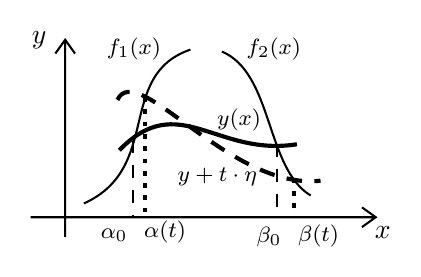
\begin{tikzpicture}[x=0.75pt,y=0.75pt,yscale=-0.95,xscale=0.95]
	%uncomment if require: \path (0,142); %set diagram left start at 0, and has height of 142
	
	%Shape: Axis 2D [id:dp8759019092999467] 
	\draw  (57,105) -- (232,105)(74.5,15) -- (74.5,115) (225,100) -- (232,105) -- (225,110) (69.5,22) -- (74.5,15) -- (79.5,22)  ;
	%Curve Lines [id:da09356767721912829] 
	\draw [line width=0.75]    (84,98) .. controls (124,80) and (100,33) .. (138,20) ;
	%Straight Lines [id:da3643716175722038] 
	\draw  [dash pattern={on 4.5pt off 4.5pt}]  (109,66) -- (109,105) ;
	%Curve Lines [id:da8219577785795169] 
	\draw [line width=0.75]    (199,94) .. controls (176,80) and (180,32) .. (154,21) ;
	%Straight Lines [id:da6076505280254729] 
	\draw  [dash pattern={on 4.5pt off 4.5pt}]  (182,68) -- (182,105) ;
	%Curve Lines [id:da05152443276483076] 
	\draw [line width=1.5]    (102,71) .. controls (132,40) and (151,74.5) .. (192,68) ;
	%Curve Lines [id:da10892530519413457] 
	\draw [line width=1.5]  [dash pattern={on 5.63pt off 4.5pt}]  (101,45.5) .. controls (111,24.5) and (158,91.5) .. (204,86.5) ;
	%Straight Lines [id:da7457157759094812] 
	\draw [line width=1.5]  [dash pattern={on 1.69pt off 2.76pt}]  (115,44) -- (115,105) ;
	%Straight Lines [id:da2336236486608474] 
	\draw [line width=1.5]  [dash pattern={on 1.69pt off 2.76pt}]  (190.5,85.5) -- (190.5,105) ;
	
	% Text Node
	\draw (91,109.4) node [anchor=north west][inner sep=0.75pt]  [font=\footnotesize]  {$\alpha _{0}$};
	% Text Node
	\draw (230,108.4) node [anchor=north west][inner sep=0.75pt]    {$x$};
	% Text Node
	\draw (56,9.4) node [anchor=north west][inner sep=0.75pt]    {$y$};
	% Text Node
	\draw (170,108.4) node [anchor=north west][inner sep=0.75pt]  [font=\footnotesize]  {$\beta _{0}$};
	% Text Node
	\draw (94,12.4) node [anchor=north west][inner sep=0.75pt]  [font=\footnotesize]  {$f_{1}( x)$};
	% Text Node
	\draw (165,12.4) node [anchor=north west][inner sep=0.75pt]  [font=\footnotesize]  {$f_{2}( x)$};
	% Text Node
	\draw (150,48.6) node [anchor=north west][inner sep=0.75pt]  [font=\footnotesize]  {$y( x)$};
	% Text Node
	\draw (130,78.6) node [anchor=north west][inner sep=0.75pt]  [font=\footnotesize]  {$y+t\cdot \eta $};
	% Text Node
	\draw (113,105.4) node [anchor=north west][inner sep=0.75pt]  [font=\footnotesize]  {$\alpha ( t)$};
	% Text Node
	\draw (191,107.4) node [anchor=north west][inner sep=0.75pt]  [font=\footnotesize]  {$\beta ( t)$};
	
	
\end{tikzpicture}
\caption{~}
\label{l3:fig:4}
\end{figure}
\noindent Таким образом 
\begin{equation*}
	\J[y+t\cdot\eta]=\int\limits_{\alpha(t)}^{\beta(t)} F(x,y+t\cdot\eta,y'+t\cdot\eta')\,dx\geqslant\J[y]=\int\limits_{\alpha_0}^{\beta_0}F(x,y,y')\,dx.
\end{equation*}
Абсолютно так же, как раньше, получим, что главная часть $\delta\J$ приращения \begin{equation*}
	\J[y+t\cdot\eta]-\J[y]=\delta\J+\ldots,
\end{equation*}  
есть
\begin{gather*}
	\delta\J=t\cdot\left.\der{}{x}\J[y+t\cdot\eta]\right|_{t=0}\text{ --- первая вариация,}\\ \intertext{и что на минимайзере}
	\delta\J=0.
\end{gather*}
Положим как обычно $\tilde{y}=y+t\cdot\eta$, $\widetilde{F}=F(x,\tilde{y},\tilde{y}')$ и найдём  выражение для $\delta\J$. Имеем 
\begin{multline}
	\label{l3:eq:20}
	\delta\J=t\cdot\left.\der{}{t}\int\limits_{\alpha(t)}^{\beta(t)}F(x,\tilde{y},\tilde{y}')\,dx\right|_{t=0}=t\cdot\Bigg\{\left.\int\limits_{\alpha(t)}^{\beta(t)}\left(\widetilde{F}_{\tilde{y}}\cdot\eta+\widetilde{F}_{\tilde{y}'}\cdot\eta'\right)\,dx\right|_{t=0}+\\+
	\Big[F\big(\beta(t),y(\beta(t))+t\cdot\eta(\beta(t)),y'(\beta(t))+t\cdot\eta'(\beta(t))\big)\cdot\beta'(t)-\\-F\big(\alpha(t),y(\alpha(t))+t\cdot\eta(\alpha(t)),y'(\alpha(t))+t\cdot\eta'(\alpha(t))\big)\cdot\alpha'(t)\Big]_{t=0}\Bigg\}=\\
	=t\cdot\Bigg\{\int\limits_{\alpha_0}^{\beta_0}\left(F_{y}\cdot\eta+F_{y'}\cdot\eta'\right)\,dx+F\big(\beta_0,y(\beta_0),y'(\beta_0)\big)\cdot\beta'(0)-\\-F\big(\alpha_0,y(\alpha_0),y'(\alpha_0)\big)\cdot\alpha'(0)\Bigg\}.
\end{multline}
Производные $\beta'(0)$ и $\alpha'(0)$ находим из равенств
\begin{gather*}
	\tilde{y}(\alpha(t))=y(\alpha(t))+t\cdot\eta(\alpha(t))=f_1(\alpha(t));\\ \tilde{y}(\beta(t))=y(\beta(t))+t\cdot\eta(\beta(t))=f_2(\beta(t)).
\end{gather*}
Продифференцируем эти равенства по $t$ и положим $t=0$. Получим
\begin{gather*}
	 y'(\alpha_0)\cdot\alpha'(0)+\eta(\alpha_0)=f'_1(\alpha_0)\cdot\alpha'(0),\\ y'(\beta_0)\cdot\beta'(0)+\eta(\beta_0)=f'_2(\beta_0)\cdot\beta'(0).
\end{gather*}
Отсюда 
\begin{equation}
	\label{l3:eq:21}
	\alpha'(0)=\frac{\eta(\alpha_0)}{f'_1(\alpha_0)-y'(\alpha_0)},\quad \beta'(0)=\frac{\eta(\beta_0)}{f'_2(\beta_0)-y'(\beta_0)}.
\end{equation}
Именно здесь мы использовали тот факт, что график минимайзера не касается граничных кривых, а их пересекает (то есть производные $f'_1(\alpha_0)\neq y'(\alpha_0)$,\ $f'_2(\beta_0)\neq y'(\beta_0)$). Далее интегрируем по частям 
\begin{equation}
	\label{l3:eq:22}
	\int\limits_{\alpha_0}^{\beta_0}\underbrace{F_{y'}}_{u}\cdot\underbrace{\eta'\,dx}_{dv}=F_{y'}\cdot\eta\mathop{\Big|}\limits_{\alpha_0}^{\beta_0}-\int\limits_{\alpha_0}^{\beta_0}\der{}{x}F_{y'}\cdot\eta\,dx.
\end{equation}
Учтём формулы \eqref{l3:eq:21}, \eqref{l3:eq:22} в выражении \eqref{l3:eq:20} для $\delta\J$ и запишем, что $\delta\J=0$
\begin{multline}
	\label{l3:eq:23}
	t\cdot\Bigg\{\int\limits_{\alpha_0}^{\beta_0}\left(F_{y}-\der{}{x}F_{y'}\right)\cdot\eta\,dx+\left.\left(F\cdot\frac{\eta}{f'_2-y'}+F_{y'}\cdot\eta\right)\right|_{x=\beta_0}-\\-\left.\left(F\cdot\frac{\eta}{f'_1-y'}+F_{y'}\cdot\eta\right)\right|_{x=\alpha_0}\Bigg\}=0.
\end{multline}
Взяв здесь $\eta(\alpha_0)=\eta(\beta_0)=0$ и применяя лемму Лагранжа получим, что минимайзер удовлетворяет уравнению Эйлера 
\begin{equation}
	\label{l3:eq:24}
	 F_{y}-\der{}{x}F_{y'}=0.
\end{equation}
Учитывая это получаем согласно \eqref{l3:eq:23} 
\begin{equation*}
	\left.\left(\frac{F}{f'_2-y'}+F_{y'}\right)\cdot\eta\right|_{x=\beta_0}-\left.\left(\frac{F}{f'_1-y'}+F_{y'}\right)\cdot\eta\right|_{x=\alpha_0}=0.
\end{equation*}
Полагая здесь $\eta(\beta_0)=1$, $\eta(\alpha_0)=0$, а потом $\eta(\beta_0)=0$, $\eta(\alpha_0)=1$ получим условия
\begin{equation}
	\label{l3:eq:25}
	 \Big(F+(f'_2-y')\cdot F_{y'}\Big)\Big|_{x=\beta_0}=0,\quad \Big(F+(f'_1-y')\cdot F_{y'}\Big)\Big|_{x=\alpha_0}=0.
\end{equation}
Условия \eqref{l3:eq:25} называются \emph{условиями трансверсальности}. Они играют ту же роль, что ЕГУ.

При решении уравнения \eqref{l3:eq:24} мы получили $y=y(x,c_1,c_2)$. Для нахождения неизвестных $c_1,\ c_2,\ \alpha_0,\ \beta_0$ у нас есть четыре условия: два в \eqref{l3:eq:25} и два условия
\begin{equation*}
	 y(\alpha_0)=f_1(\alpha_0),\ y(\beta_0)=f_2(\beta_0).
\end{equation*}

\noindent\textbf{Задание. }Пусть $F(x,y,y')=A(x,y)\cdot\sqrt{1+y^{\prime2}}$ и $A(x,y)>0$. Докажите, что в этом случае условия трансверсальности переходят в условия ортогональности. 